\chapter{Reference Manual}
\label{chpt:ReferenceManual}
\typeout{$Id$}

\begin{figure}[hbpt]
\begin{centering}
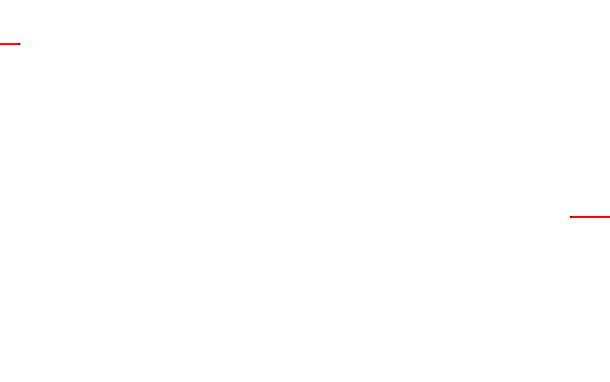
\includegraphics[width=5in]{MainWindowAnnotated.png}
\caption{Main Window, Annotated.}
\label{ref:fig:mainwindow}
\end{centering}
\end{figure}
\begin{table}[hbpt]
\begin{centering}
\begin{tabular}{|l|p{3in}|}
\hline
Menu Item & Description \\
\hline
\hline
Clear & Clear the main text area. \\
\hline
Save As\ldots & Save the main text area as a text file. \\
\hline
Print\ldots & Print the main text area on a printer. \\
\hline
Reload Menu & Reload and rebuild the commands menu. \\
\hline
Quit & Quit the application (and log out of your X11  session). \\
\hline
\end{tabular}
\caption{Session menu}
\label{ref:tab:sessionmenu}
\end{centering}
\end{table}
The annotated main window for the TkSessionManager is shown in
Figure~\ref{ref:fig:mainwindow}.  There is a menu bar along the top,
with five menus: \texttt{Session}, \texttt{Edit}, \texttt{Commands}, 
\texttt{Actions}, and \texttt{Help}.  The \texttt{Session} contains menu
item to clear the text area, save the main text area as a text file,
print the main text area on a printer, reload the menu file, and quit
the application\footnote{If TkSessionManager is the last or only command
in your .xinitrc or .xsession file, this will in fact quit your X11
session.}, as described in Table~\ref{ref:tab:sessionmenu}.


\begin{table}[hbpt]
\begin{centering}
\begin{tabular}{|l|p{3in}|}
\hline
Menu Item & Description \\
\hline
\hline
Undo & Undo last change.  Not used. \\
\hline
Cut & Cut selection to the paste buffer. \\
\hline
Copy & Copy selection to the paste buffer. \\
\hline
Paste & Paste in the paste buffer. \\
\hline
Clear & Clear selection. \\
\hline
Delete & Delete selection. \\
\hline
Select All & Select everything. \\
\hline
De-select All & Select nothing. \\
\hline
Preferences & Edit Preferences. \\
\hline
Menu & Edit Menu. \\
\hline
\end{tabular}
\caption{Edit menu}
\label{ref:tab:editmenu}
\end{centering}
\end{table}
The \texttt{Edit} menu contains, in addition to the standard edit
functions of cut; copy; paste; clear; delete; select all; deselect all,
menu items to edit the preferences (see
Section~\ref{sect:ItemProperties}) and the commands menu (see
Section~\ref{sect:EditCommandMenu}), as described in Table~\ref{ref:tab:editmenu}.

The \texttt{Commands} menu is completely user defined.  This menu is
built from the contents of the specified menu file.  See
Section~\ref{sect:CommandMenuFile} for a detailed description of this
file.

\begin{table}[hbpt]
\begin{centering}
\begin{tabular}{|l|p{3in}|}
\hline
Menu Item & Description \\   
\hline
\hline
Suspend & Suspend to RAM. \\
\hline
Hibernate & Hibername to disk. \\
\hline
\end{tabular}
\caption{Actions menu}
\label{ref:tab:actionsmenu}
\end{centering}
\end{table}
The \texttt{Actions} menu has menu items for controlling the system as a
whole. This includes suspending and hibernating the system, as shown in
Table~\ref{ref:tab:actionsmenu}. 

\begin{table}[hbpt]
\begin{centering}
\begin{tabular}{|l|p{3in}|}
\hline
Menu Item & Description \\
\hline
\hline
On Help\ldots & Help about the help viewer. \\
\hline
Tutorial\ldots & A tutorial for the TkSessionManager program.\\
\hline
On Version & Show the running version of the TkSessionManager.\\
\hline
Warranty & Show warranty information.\\
\hline
Copying & Show copying information.\\
\hline
Reference Manual & Show the detailed reference manual.\\
\hline
\end{tabular}
\caption{Help menu}
\label{ref:tab:helpmenu}
\end{centering}
\end{table}
Finally, the \texttt{Help} menu has menu items for accessing this
document on-line, as shown in Table~\ref{ref:tab:helpmenu}.

\section{Command Menu File format}
\label{sect:CommandMenuFile}

The menu file consists of pairs of lines, the menu item text and the
command to run (which should be something suitable as an argument list
to the Tcl exec command).  Lines starting with a `!' are comments and
ignored. A casscade is introduced by using a `\{' at the beginning of the
menu item text.  Lines are processed as menu items under the casscade
name until a lone `\}' on a line by itself.  Casscades can occur under
casscades.  There is no set limit to the depth casscades can go.

Commands are passed to the Tcl \texttt{exec} command and always forked
as background tasks, with a \& added to the end of the command and the
command's stdout and stderr bound to the pipe feeding to the text area.
A simple sample menu file is shown in Listing~\ref{ref:lst:sample}.
This menu defings the menu items \texttt{Terminal}, \texttt{GnuEmacs},
\texttt{CS Machines} (a cascade menu), \texttt{Gimp},
\texttt{Inkscape}, \texttt{Audacity}, and \texttt{Kino}.  The
\texttt{CS Machines} cascade menu has two items, \texttt{Foo} and
\texttt{Bar}. Each of the items is followed by the command line to run.
For example the \texttt{Terminal} menu item runs the command
\texttt{/usr/bin/xterm}, which launches the old-school xterm program,
which opens up a shell window.  The two menu items under the \texttt{CS
Machines} cascade also open up xterm windows, but use slogin to log in
remotely to machines on the CS network at \texttt{school.edu}.

\begin{lstlisting}[caption={Sample Menu},label=ref:lst:sample]
! Sample menu
Terminal
/usr/bin/xterm
GnuEmacs
/usr/bin/emacs
{CS Machines
Foo
/usr/bin/xterm -title Foo -n Foo -e slogin foo.cs.school.edu
Bar
/usr/bin/xterm -title Bar -n Bar -e slogin bar.cs.school.edu
}
Gimp
/usr/bin/gimp
Inkscape
/usr/bin/inkscape
Audacity
/usr/bin/audacity
Kino
/usr/bin/kino
\end{lstlisting}

While it is quite possible to ``hand edit'' this file using your
favorite plain text editor, the TkSessionManager program includes a
simple built in editing tool, which is described in
Section~\ref{sect:EditCommandMenu}.

\section{Edit Command Menu}
\label{sect:EditCommandMenu}

\begin{figure}[hbpt] 
\begin{centering}
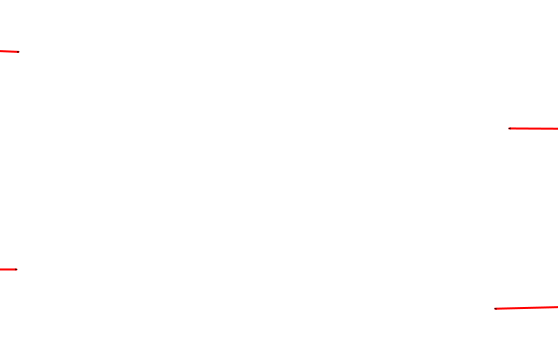
\includegraphics[width=5in]{MenuEditorAnnotated.png} 
\caption{Menu Editor Window, annotated.} 
\label{ref:fig:menueditor} 
\end{centering}
\end{figure}
The annotated Menu Editor window for the TkSessionManager is shown in
Figure~\ref{ref:fig:menueditor}. At the top is the name of the menu
filename to save in, in the middle is the menu displayed as a tree,
with a set of four edit command buttons just below the menu tree, and a
set of dialog control buttons at the bottom.  There are buttons for
inserting new commands and cascades, a button to delete a command or
cascade, and a button for showing (and editing) the properties of a
command or cascade.  

\begin{figure}[hbpt] 
\begin{centering}

\includegraphics{CommandPropertiesAnnotated.png} 
\caption{Command Properties window, annotated.} 
\label{ref:fig:commandprop} 
\end{centering}
\end{figure}
\begin{figure}[hbpt] 
\begin{centering}
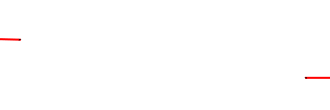
\includegraphics{CasscadePropertiesAnnotated.png} 
\caption{Casscade Properties window, annotated.} 
\label{ref:fig:cascadeprop} 
\end{centering}
\end{figure}
The two insert buttons and the properites button
all pop up a small properties window, show in
Figures~\ref{ref:fig:commandprop} and Figures~\ref{ref:fig:cascadeprop}.
In both windows, there is an editable text label and in the case of the
command properties window, there is a command path that can be edited.
The edits in these windows can be saved by clicking the OK button or the
changes can be discarded by clicking the Cancel button.



\section{Item Properties}
\label{sect:ItemProperties}

\begin{figure}[hbpt]
\begin{centering}
\includegraphics[width=5in]{PreferencesEditor.png}
\caption{Preferences Editor Window.}
\label{ref:fig:preferenceseditor}
\end{centering}
\end{figure}



